\documentclass[a4paper, 12pt]{article}%тип документа

%%%Библиотеки
	%\usepackage[warn]{mathtext}	
	\usepackage[T2A]{fontenc} % кодировка
	\usepackage[utf8]{inputenc} % кодировка исходного текста
	\usepackage[english,russian]{babel} % локализация и переносы
	\usepackage{caption}
	\usepackage{listings}
	\usepackage{amsmath,amsfonts,amssymb,amsthm,mathtools}
	\usepackage{wasysym}
	\usepackage{graphicx}%Вставка картинок правильная
	\usepackage{float}%"Плавающие" картинки
	\usepackage{wrapfig}%Обтекание фигур (таблиц, картинок и прочего)
	\usepackage{fancyhdr} %загрузим пакет
	\usepackage{lscape}
	\usepackage{xcolor}
	\usepackage[normalem]{ulem}
	\usepackage{hyperref}

%%%Конец библиотек




%%%Настройка ссылок
	\hypersetup
	{
		colorlinks=true,
		linkcolor=blue,
		filecolor=magenta,
		urlcolor=blue
	}
%%%Конец настройки ссылок


%%%Настройка колонтитулы
	\pagestyle{fancy}
	\fancyhead{}
	\fancyhead[L]{Лабораторная работа}
	\fancyhead[R]{Талашкевич Даниил, группа Б01-008}
	\fancyfoot[C]{\thepage}
%%%конец настройки колонтитулы



							\begin{document}
						%%%%Начало документа%%%%


%%%Начало титульника
\begin{titlepage}

	\newpage
	\begin{center}
		\normalsize Московский физико-технический институт \\(госудраственный 			университет)
	\end{center}

	\vspace{6em}

	\begin{center}
		\Large Лабораторная работа по квантовой физике\\
	\end{center}

	\vspace{1em}

	\begin{center}
		\large \textbf{Изучение спектров атомов водорода и йода  [2.2]}
	\end{center}

	\vspace{2em}

	\begin{center}
		\large Талашкевич Даниил Александрович\\
		Группа Б01-008
	\end{center}

	\vspace{\fill}

	\begin{center}
	Долгопрудный \\2022
	\end{center}
	
\end{titlepage}
%%%Конец Титульника



%%%Настройка оглавления и нумерации страниц
	\thispagestyle{empty}
	\newpage
	\tableofcontents
	\newpage
	\setcounter{page}{1}
%%%Настройка оглавления и нумерации страниц


					%%%%%%Начало работы с текстом%%%%%%



\section{Аннотация}

\textbf{В работе исследуются}: сериальные закономерости в оптическом спектре водорода; спектр поглощения паров йода в видимой области.

\subsection{Теория}

Длины волн спектральных линий водородоподобного атома описываются формулой
\begin{equation}
\dfrac{1}{\lambda_{mn}} = RZ^2 \left( \dfrac{1}{n^2} - \dfrac{1}{m^2} \right),
\end{equation}
\begin{wrapfigure}{r}{0.4\textwidth}
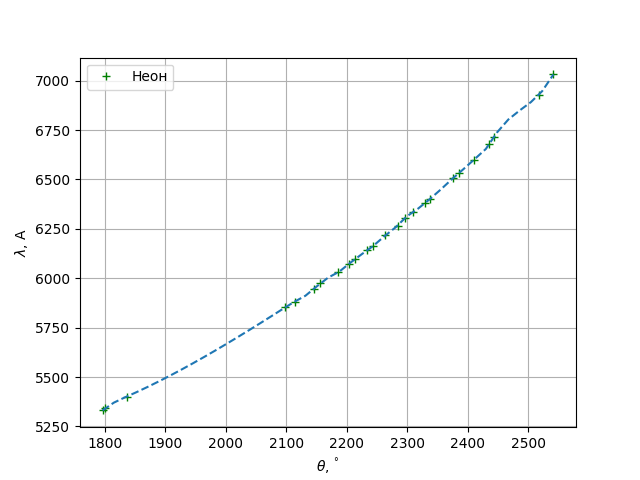
\includegraphics[width = 0.37\textwidth]{1.png}
\centering
\caption{Линии молекулы йода.}
\end{wrapfigure}
где $R = 109677.6~\text{см}^{-1}$ -- константа, называемая постоянной Ридберга, а $m$ и $n$ -- целые числа. Мы будем изучать серию Бальмера, линии которой лежат в видимой области. Для неё $n = 2$, а $m = 3,~4,~5,~6\dots$ Первые четыре линии обозначаются соответственно $H_\alpha$, $H_\beta$, $H_\gamma$, $H_\delta$.
Для молекулы йода мы рассматриваем только нулевую серию, энергетическое положение линий поглощения определяется выражением
\begin{equation}
h\nu_{0, n_2} = (E_2 - E_1) + h\nu_2 \left( n_2 + \dfrac{1}{2} \right) - \dfrac{1}{2} h \nu_1.
\end{equation}

\subsection{Описание установки}

Для наблюдения спектра водорода используется установка, изображённая на Рис. 2А. Источником света для наблюдения служит водородная трубка Н-образной формы, в состав газа которой добавлены водные пары для увеличения яркости интересующих нас линий. Источник Л помещается на оптическую скамью вместе с конденсером К, так что свет концентрируется на входной щели 1. Далее через коллиматорный объектив 2 свет попадает на сложную спектральную призму, состояющую из призм П$_1$, П$_2$ и П$_3$. Первые две призмы обладают большой дисперсией, а промежуточная П$_3$ поворачивает лучи -- такое устройство позволяет складывать дисперии П$_1$ и П$_2$. После прохождения призмы свет попадает в зрительную трубу 4-5, объектив которой даёт изображение входной щели различных цветов.
\newpage
\begin{figure}[h]
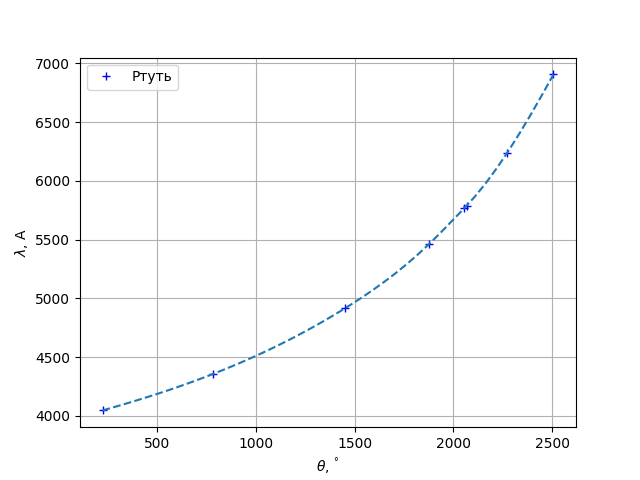
\includegraphics[scale=0.5]{2.png}
\centering
\caption{Установки для наблюдения линий А. водорода; Б. йода.}
\end{figure} 
На Рис. 2Б изображена схема установки, используемой для наблюдения спектра йода. Спектр поглощения паров йода наблюдается визуально на фоне сплошного спектра лампы накаливания 1, питаемой от блока питания 2. Кювета 3 с кристаллами йода подогревается нихромовой спиралью, подключённой вместе с лампой накаливания к блоку питания. Линза 4 используется как конденсор. В результате подогрева кристаллы йода частично возгоняются, образуя пары
с лёгкой фиолетовой окраской. Спектрометр 5 позволяет визуально наблюдать линии поглощения молекул йода на фоне сплошного спектра излучения лампы накаливания видимой области.

\section{Ход работы}

\subsection{Градуировка}

Снимем зависимость длины волны света от параметра $ \theta $ барабана монохроматора. Погрешность $ \sigma_\theta = 5 ^\circ $. Результаты занесем в таблицу:
	\begin{table}[H]
		\begin{center}
			\resizebox{\columnwidth}{!}{%
				\begin{tabular}{|rrr|rrrrrr}
					\cline{1-3} \cline{7-9}
					\multicolumn{3}{|c|}{Неон}                                                                                                &                      &                      & \multicolumn{1}{r|}{} & \multicolumn{3}{c|}{Ртуть}                                                                                               \\ \cline{1-3} \cline{7-9} \multicolumn{1}{|c|}{} & \multicolumn{1}{c|}{} & \multicolumn{1}{c|}{} & \multicolumn{1}{c}{} & \multicolumn{1}{c}{} & \multicolumn{1}{c|}{} & \multicolumn{1}{c|}{} & \multicolumn{1}{c|}{} & \multicolumn{1}{c|}{} \\ 
					\multicolumn{1}{|c|}{Линия} & \multicolumn{1}{c|}{Угол $\theta ^\circ$} & \multicolumn{1}{c|}{Длина волны, \AA} & \multicolumn{1}{c}{} & \multicolumn{1}{c}{} & \multicolumn{1}{c|}{} & \multicolumn{1}{c|}{Линия} & \multicolumn{1}{c|}{Угол $\theta ^\circ$} & \multicolumn{1}{c|}{Длина волны, \AA} \\ \cline{1-3} \cline{7-9} 
					\multicolumn{1}{|r|}{1}     & \multicolumn{1}{r|}{2542}            & 7032                                                 &                      &                      & \multicolumn{1}{r|}{} & \multicolumn{1}{r|}{K1}    & \multicolumn{1}{r|}{2506}            & \multicolumn{1}{r|}{6907}                            \\ \cline{1-3} \cline{7-9} 
					\multicolumn{1}{|r|}{2}     & \multicolumn{1}{r|}{2518}            & 6929                                                 &                      &                      & \multicolumn{1}{r|}{} & \multicolumn{1}{r|}{K2}    & \multicolumn{1}{r|}{2270}            & \multicolumn{1}{r|}{6234}                            \\ \cline{1-3} \cline{7-9} 
					\multicolumn{1}{|r|}{3}     & \multicolumn{1}{r|}{2444}            & 6717                                                 &                      &                      & \multicolumn{1}{r|}{} & \multicolumn{1}{r|}{1}     & \multicolumn{1}{r|}{2068}            & \multicolumn{1}{r|}{5791}                            \\ \cline{1-3} \cline{7-9} 
					\multicolumn{1}{|r|}{4}     & \multicolumn{1}{r|}{2436}            & 6678                                                 &                      &                      & \multicolumn{1}{r|}{} & \multicolumn{1}{r|}{2}     & \multicolumn{1}{r|}{2056}            & \multicolumn{1}{r|}{5770}                            \\ \cline{1-3} \cline{7-9} 
					\multicolumn{1}{|r|}{5}     & \multicolumn{1}{r|}{2410}            & 6599                                                 &                      &                      & \multicolumn{1}{r|}{} & \multicolumn{1}{r|}{3}     & \multicolumn{1}{r|}{1876}            & \multicolumn{1}{r|}{5461}                            \\ \cline{1-3} \cline{7-9} 
					\multicolumn{1}{|r|}{6}     & \multicolumn{1}{r|}{2386}            & 6533                                                 &                      &                      & \multicolumn{1}{r|}{} & \multicolumn{1}{r|}{4}     & \multicolumn{1}{r|}{1452}            & \multicolumn{1}{r|}{4916}                            \\ \cline{1-3} \cline{7-9} 
					\multicolumn{1}{|r|}{7}     & \multicolumn{1}{r|}{2376}            & 6507                                                 &                      &                      & \multicolumn{1}{r|}{} & \multicolumn{1}{r|}{5}     & \multicolumn{1}{r|}{786}             & \multicolumn{1}{r|}{4358}                            \\ \cline{1-3} \cline{7-9} 
					\multicolumn{1}{|r|}{8}     & \multicolumn{1}{r|}{2338}            & 6402                                                 &                      &                      & \multicolumn{1}{r|}{} & \multicolumn{1}{r|}{6}     & \multicolumn{1}{r|}{226}             & \multicolumn{1}{r|}{4047}                            \\ \cline{1-3} \cline{7-9} 
					\multicolumn{1}{|r|}{9}     & \multicolumn{1}{r|}{2330}            & 6383                                                 &                      &                      &                       &                            &                                      &                                                      \\ \cline{1-3}
					\multicolumn{1}{|r|}{10}    & \multicolumn{1}{r|}{2310}            & 6334                                                 &                      &                      &                       &                            &                                      &                                                      \\ \cline{1-3}
					\multicolumn{1}{|r|}{11}    & \multicolumn{1}{r|}{2296}            & 6305                                                 &                      &                      &                       &                            &                                      &                                                      \\ \cline{1-3}
					\multicolumn{1}{|r|}{12}    & \multicolumn{1}{r|}{2284}            & 6267                                                 &                      &                      &                       &                            &                                      &                                                      \\ \cline{1-3}
					\multicolumn{1}{|r|}{13}    & \multicolumn{1}{r|}{2264}            & 6217                                                 &                      &                      &                       &                            &                                      &                                                      \\ \cline{1-3}
					\multicolumn{1}{|r|}{14}    & \multicolumn{1}{r|}{2244}            & 6164                                                 &                      &                      &                       &                            &                                      &                                                      \\ \cline{1-3}
					\multicolumn{1}{|r|}{15}    & \multicolumn{1}{r|}{2234}            & 6143                                                 &                      &                      &                       &                            &                                      &                                                      \\ \cline{1-3}
					\multicolumn{1}{|r|}{16}    & \multicolumn{1}{r|}{2214}            & 6096                                                 &                      &                      &                       &                            &                                      &                                                      \\ \cline{1-3}
					\multicolumn{1}{|r|}{17}    & \multicolumn{1}{r|}{2204}            & 6074                                                 &                      &                      &                       &                            &                                      &                                                      \\ \cline{1-3}
					\multicolumn{1}{|r|}{18}    & \multicolumn{1}{r|}{2186}            & 6030                                                 &                      &                      &                       &                            &                                      &                                                      \\ \cline{1-3}
					\multicolumn{1}{|r|}{19}    & \multicolumn{1}{r|}{2156}            & 5976                                                 &                      &                      &                       &                            &                                      &                                                      \\ \cline{1-3}
					\multicolumn{1}{|r|}{20}    & \multicolumn{1}{r|}{2146}            & 5945                                                 &                      &                      &                       &                            &                                      &                                                      \\ \cline{1-3}
					\multicolumn{1}{|r|}{21}    & \multicolumn{1}{r|}{2114}            & 5882                                                 &                      &                      &                       &                            &                                      &                                                      \\ \cline{1-3}
					\multicolumn{1}{|r|}{22}    & \multicolumn{1}{r|}{2098}            & 5852                                                 &                      &                      &                       &                            &                                      &                                                      \\ \cline{1-3}
					\multicolumn{1}{|r|}{23}    & \multicolumn{1}{r|}{1836}            & 5401                                                 &                      &                      &                       &                            &                                      &                                                      \\ \cline{1-3}
					\multicolumn{1}{|r|}{24}    & \multicolumn{1}{r|}{1800}            & 5341                                                 &                      &                      &                       &                            &                                      &                                                      \\ \cline{1-3}
					\multicolumn{1}{|r|}{25}    & \multicolumn{1}{r|}{1796}            & 5331                                                 &                      &                      &                       &                            &                                      &                                                      \\ \cline{1-3}
				\end{tabular}%
			} 
		\end{center}
		\caption{Градуировка монохроматора}
		\label{table g}
	\end{table}

Построим график зависимости, профитировав функцию $ \lambda (\theta) $ по дисперсионной формуле Гартмана:
	
	\begin{equation}\label{labda(thta)}
	\lambda = \lambda_0 + \dfrac{C}{\theta - \theta_0}
	\end{equation}
	
\newpage	
	
	\begin{figure*}[ht!]
            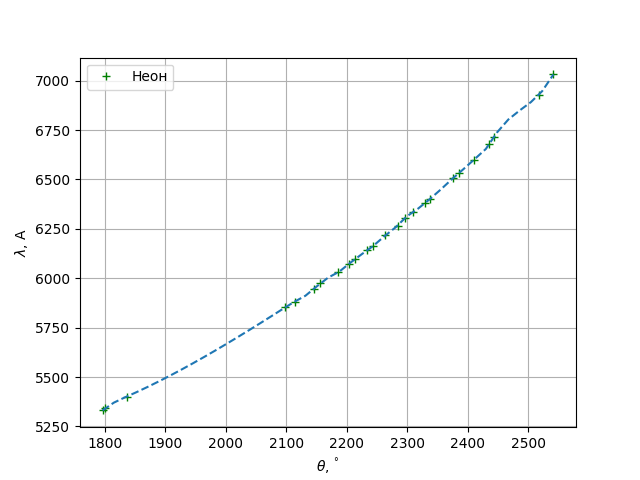
\includegraphics[width=.6\textwidth]{1.png}\hfill
            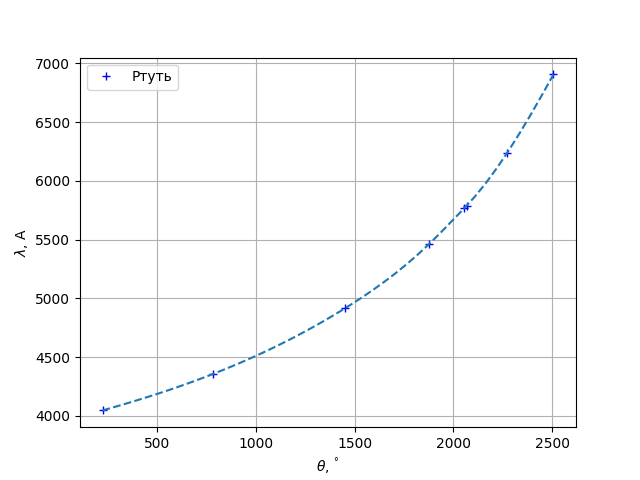
\includegraphics[width=.6\textwidth]{2.png}\hfill
            \caption{Неон}
            \caption{Ртуть}
        \end{figure*}
	
	\begin{figure}[h!]
		%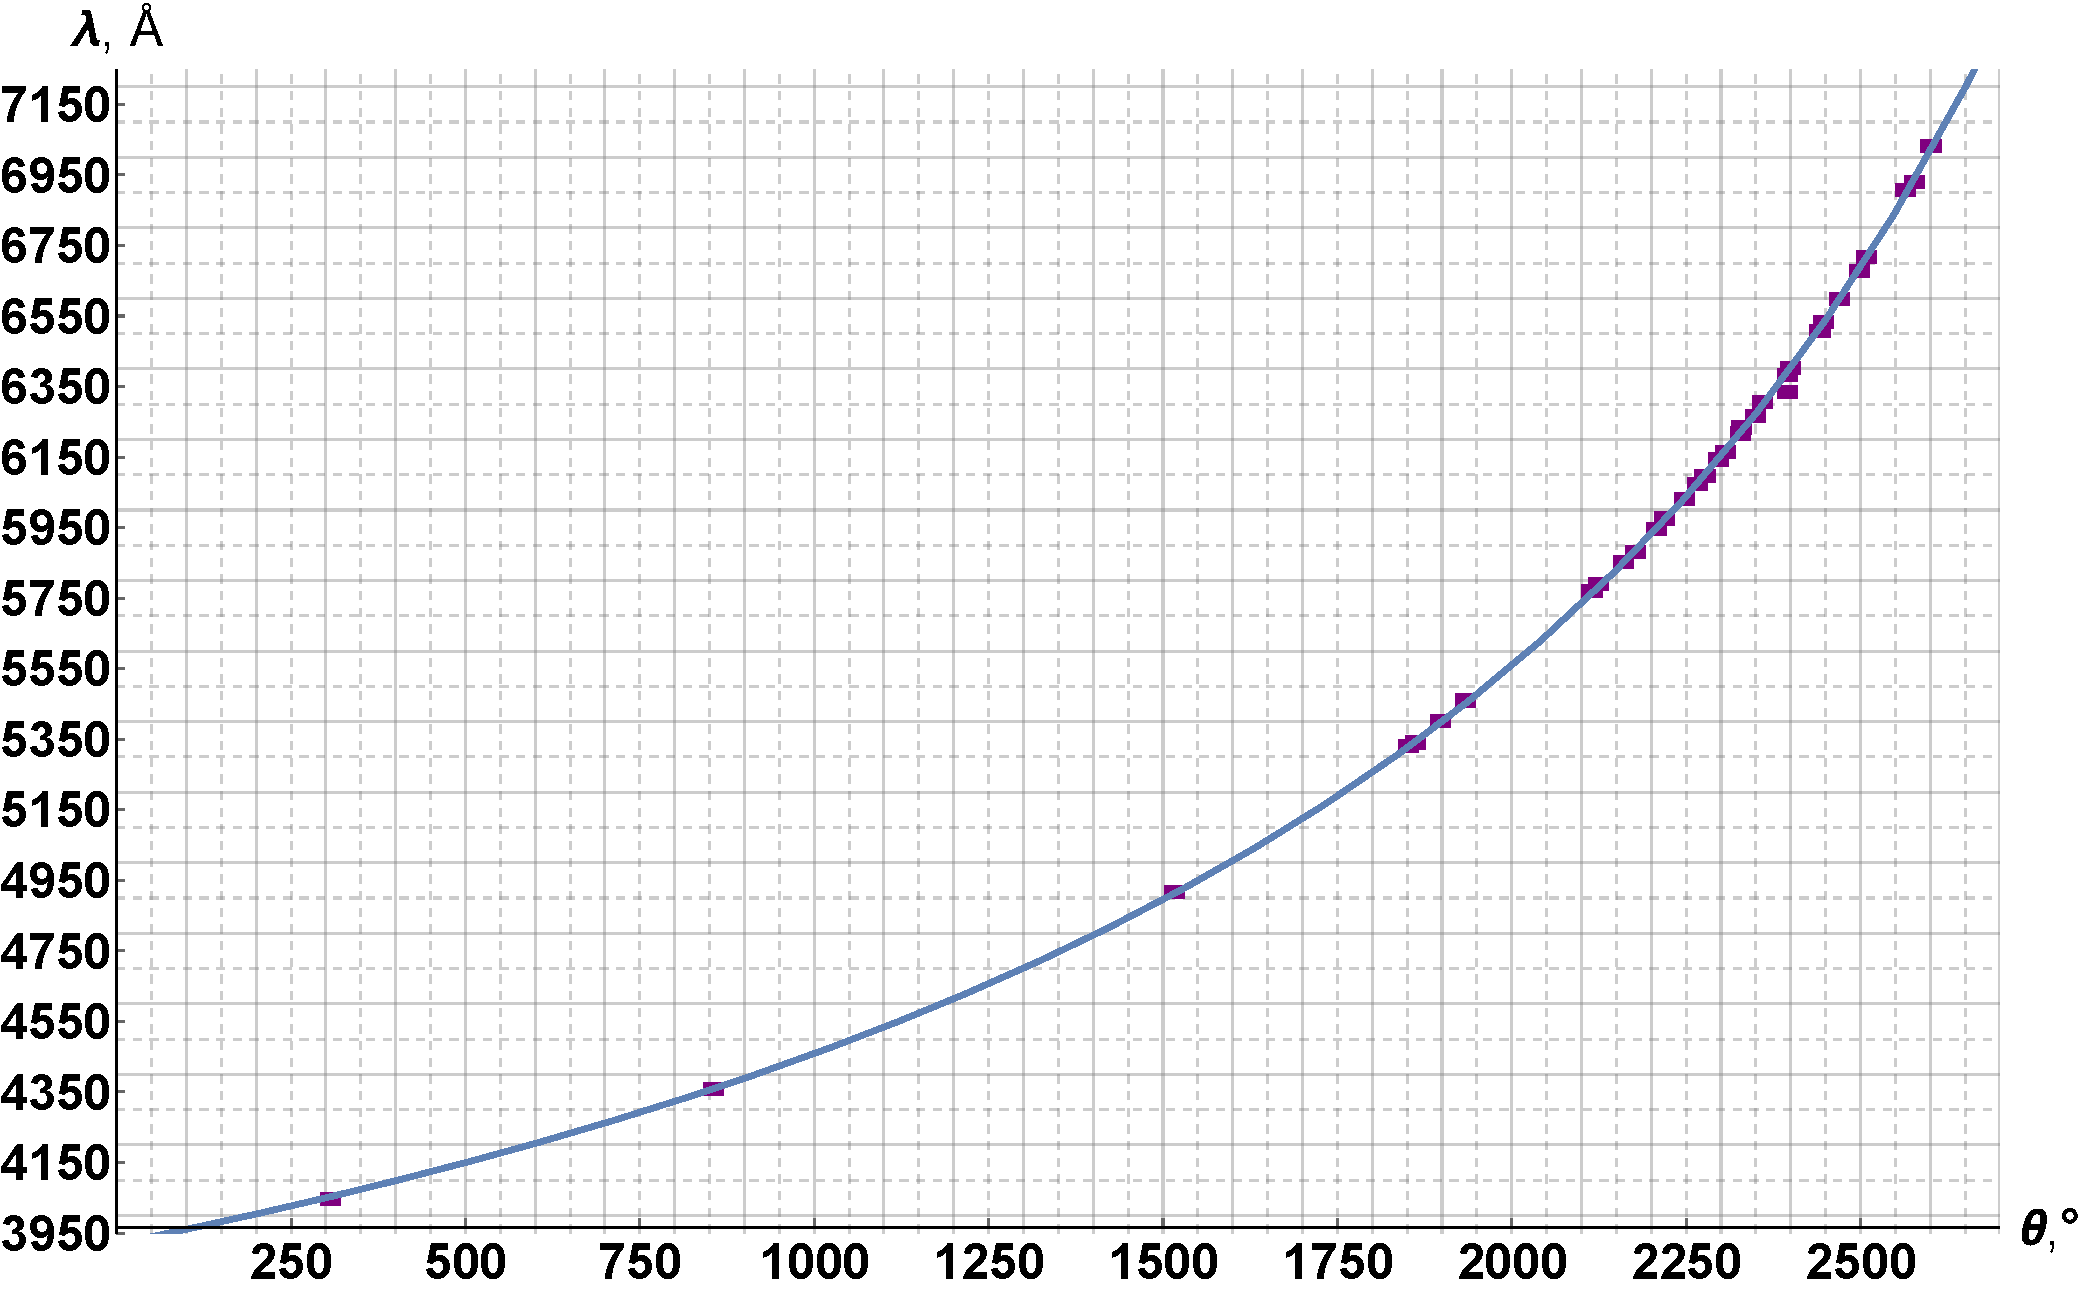
\includegraphics[scale=0.5]{G.pdf}
		\caption{Градуировка монохроматора}
		\label{graf_g}
	\end{figure} 
	
	\begin{table}[H]
		\begin{center}
			\begin{tabular}{|c|c|c|}
\hline & Значение & Ошибка \\
\hline$C[A \cdot 10^6]$ & $-6.19$ & $0.13$ \\
\hline$\theta_0\left[^{\circ}\right]$ & 3863 & 3 \\
\hline$\lambda_0[A]$ & 2342 & 5 \\
\hline
\end{tabular}
		\caption{константы для дисперсионной формулы Гертмана}
		\end{center}
		\label{}
	\end{table}

\subsection{Спектр водорода}

	Рассмотрим линии спектра водорода, опеределим их длины волн по градуировочной кривой и рассчитаем постоянную Ридберга для каждой линии.
	
	\newpage
	
		\begin{table}[h!]
		\begin{center}
			\begin{tabular}{|c|c|c|c|c|c|c|c|}
				\hline 
				Линия спектра & $ \theta $, $ ^\circ $ & $ \lambda, \;\mathring{A} $ & $ \sigma_{\lambda} $ & $ \frac{1}{n^2} - \frac{1}{m^2} $ & $ \frac{1}{\lambda}, \;  10^{-4} \mathring{A}^{-1} $  &  $ \sigma_{\frac{1}{\lambda}}, 10^{-4} \mathring{A}^{-1} $ \\ 
			\hline $ H_\alpha $ & 2396 & 6562 & 16 & 0.139 & 1.528 & 0.046 & 109757 \\
		\hline $ H_\beta $  & 1405 & 4863 & 8 & 0.188 & 2.059 & 0.062 & 109680\\
			\hline $ H_\gamma $ & 757 & 4339 & 6 & 0.21 & 2.3 & 0.069 & 109773\\
			\hline $ H_\delta $ & 338 & 4102 & 6 & 0.222 & 2.436 & 0.073 & 109736\\
				\hline 
			\end{tabular} 
		\end{center}
		\caption{Определение линий спектра водорода}
		\label{table_mn}
	\end{table}
	
	Построим график связи длины волны и номера перехода:

	\begin{figure}[!h]
		\begin{center}
		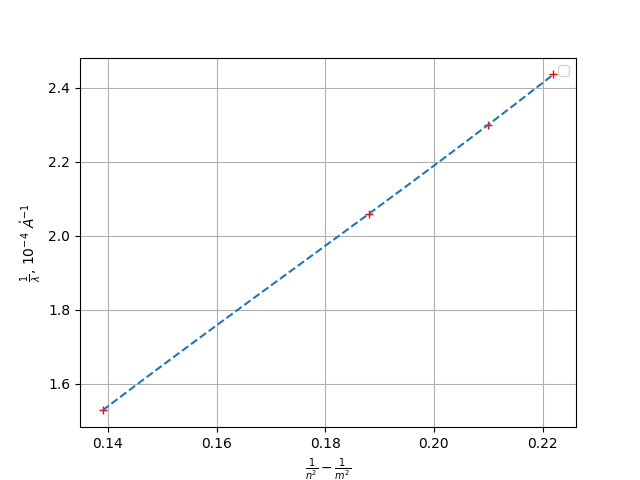
\includegraphics[scale=0.9]{3.png}
		\end{center}		
		\caption{Проверка формулы Бальмера}
		\label{graf_mn}
	\end{figure} 
	
	\begin{table}[!h]
		\begin{center}
			\begin{tabular}{|c|c|c|}
				\hline
				& \text{Значение} & \text{Погрешность} \\
				\hline
				 $ b $ & 0.0170 & 0.0053 \\
				$ a $& 10.9737 & 0.0105 \\
				\hline 
			\end{tabular} 
		\end{center}
		\caption{Фит рис. \ref{graf_mn} функцией $ y = ax +b $}
%		\label{}
	\end{table}

\newpage

	Отсюда можно определить постоянную Ридберга 
	
\begin{equation}\label{}
	R = (109737 \pm 105) \; \text{см}^{-1} 
\end{equation}
	
	\section{Вывод }
	
	Мы изучили спектры в оптических спектрах водорода и йода, экспериментально проверили справедливость формулы Бальмера и нашли постоянную Ридберга, которая в пределах погрешность совпадает с табличной ($ R = 109 677,6 \; \text{см}^{-1} $), и оценили энергии квантов возбужденного состояния молекулы, энергию диссоциации частиц и энергию электронного перехода.

\end{document}
